\section{Time Dilation and Length Contraction}
%By Matt Trawick.
\label{time_dilation_lab}

\instructornote{%
By Matt Trawick, 2019.  Time: 60 minutes?

(Activities 1 and 2 are based on a lab I did in Modern Physics for several years.)  

Activity 1 assumes that students have already seen the idea of time dilation and the Lorentz factor $\gamma$, probably by analyzing this exact situation with Anna, Bob, a train, and a flashlight.  This exercise can be their first opportunity to run with this idea a bit on their own, and introduces them to the idea of proper time.

Activity 2 is designed to be a first introduction to the idea of length contraction, showing that it follows directly from time dilation.  It also introduces the idea of proper length.

Activity 3 is an exercise involving the lifetime of muons created in the atmosphere, a classic piece of experimental evidence for time dilation.  It considers the journey through the atmosphere from the reference frames of the Earth and the muons, giving practice in both time dilation and length contraction.  Answers: (a) $1.43 \times 10^{-5}$~sec (b)~0.15\% (d)~$5.3 \times 10^{-6}$~sec (e) 9.1\% 

Depending what you want to cover, it would also be totally reasonable to do only activity 1, or only activities 1 and 2.
}

\makelabheader %(Space for student name, etc., defined in master.tex)

\bigskip

\begin{wrapfigure}[5]{r}{0.35\textwidth}
\begin{center}
\vspace{-0.3in}
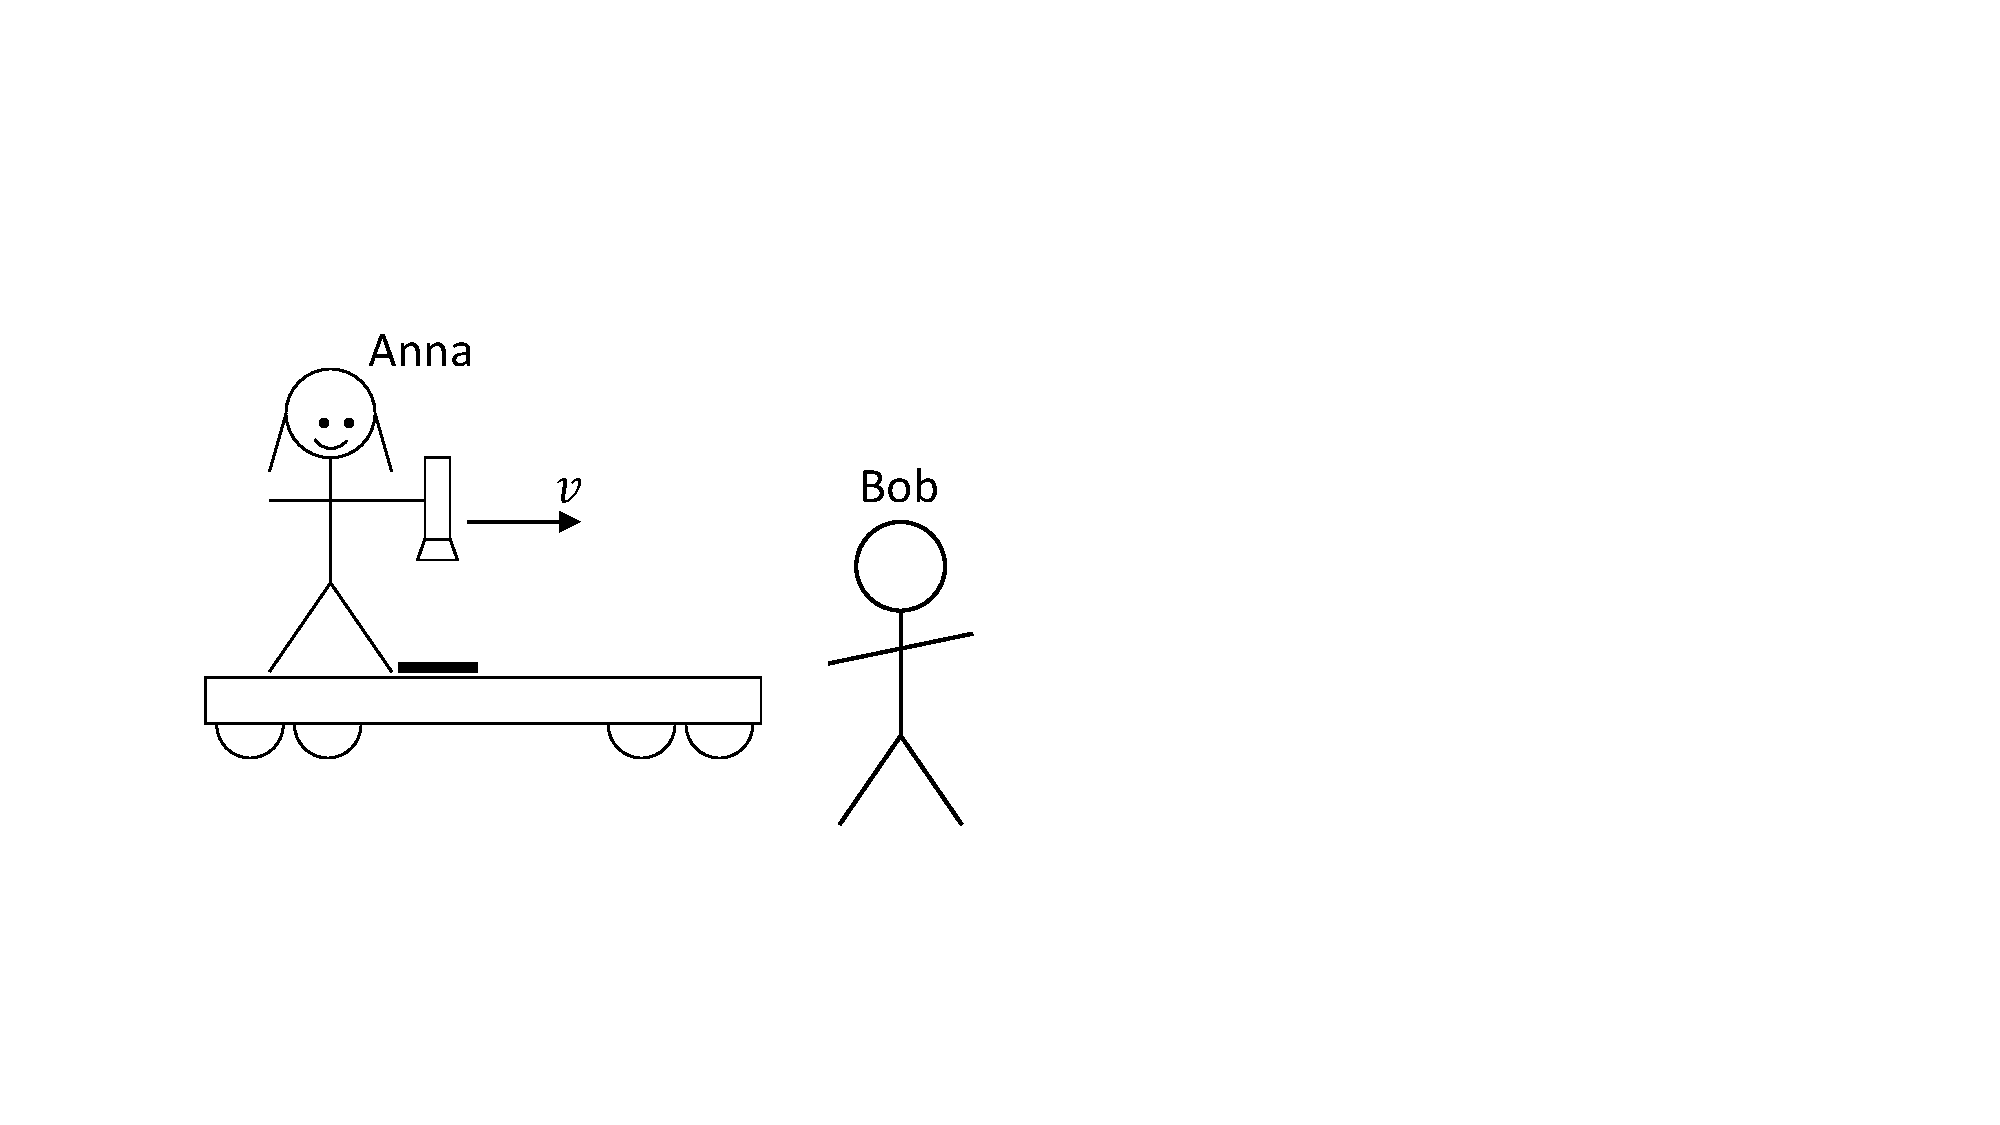
\includegraphics[scale=0.4]{time_dilation_length_contraction/anna_and_bob.pdf}
\end{center}
\end{wrapfigure}

\textbf{Activity 1: Time Dilation}

%Consider the case of Anna and Bob that we talked about in class, shown in figures 2.5 and 2.6 on page 10 of Harris.  Suppose that the train is traveling with a speed $v$ such that $\gamma=1.5$.
Anna rides a train towards the east at a speed $v$ such that $\gamma=1.5$.  She turns on a flashlight, which shines onto a mirror directly below it.

\begin{enumerate}[labparts]
\item If Anna measures the light's round trip time to be 6 nanoseconds, what does Bob measure?
\answerspace{0.5in}
\end{enumerate}

\begin{enumerate}[labparts, nosep, resume]
\item Now Anna and Bob try a variation of the experiment.  Anna rides on the train, as before, and the train moves east again, at the same speed $v$, so that $\gamma=1.5$.  But this time Bob holds the flashlight and the mirror.  Both Anna and Bob time the round trip.  What do Anna and Bob each measure for the round trip time $\Delta t$?
\answerspace{0.5in}

\item In an experiment like what Anna and Bob are doing, the shortest measured time between two events (like the emission and detection of a photon) is called the ``proper time.''  What determines who measures the shortest time? Is it who's on the train?  Is it who holds the flashlight?  Is it who holds the mirror?
\answerspace{0.5in}

\item Write a definition of the \textit{proper time,} $\Delta t_0$, between two events.
\answerspace{0.5in}
\end{enumerate}

\begin{wrapfigure}[7]{r}{0.35\textwidth}
\begin{center}
\vspace{-0.4in}
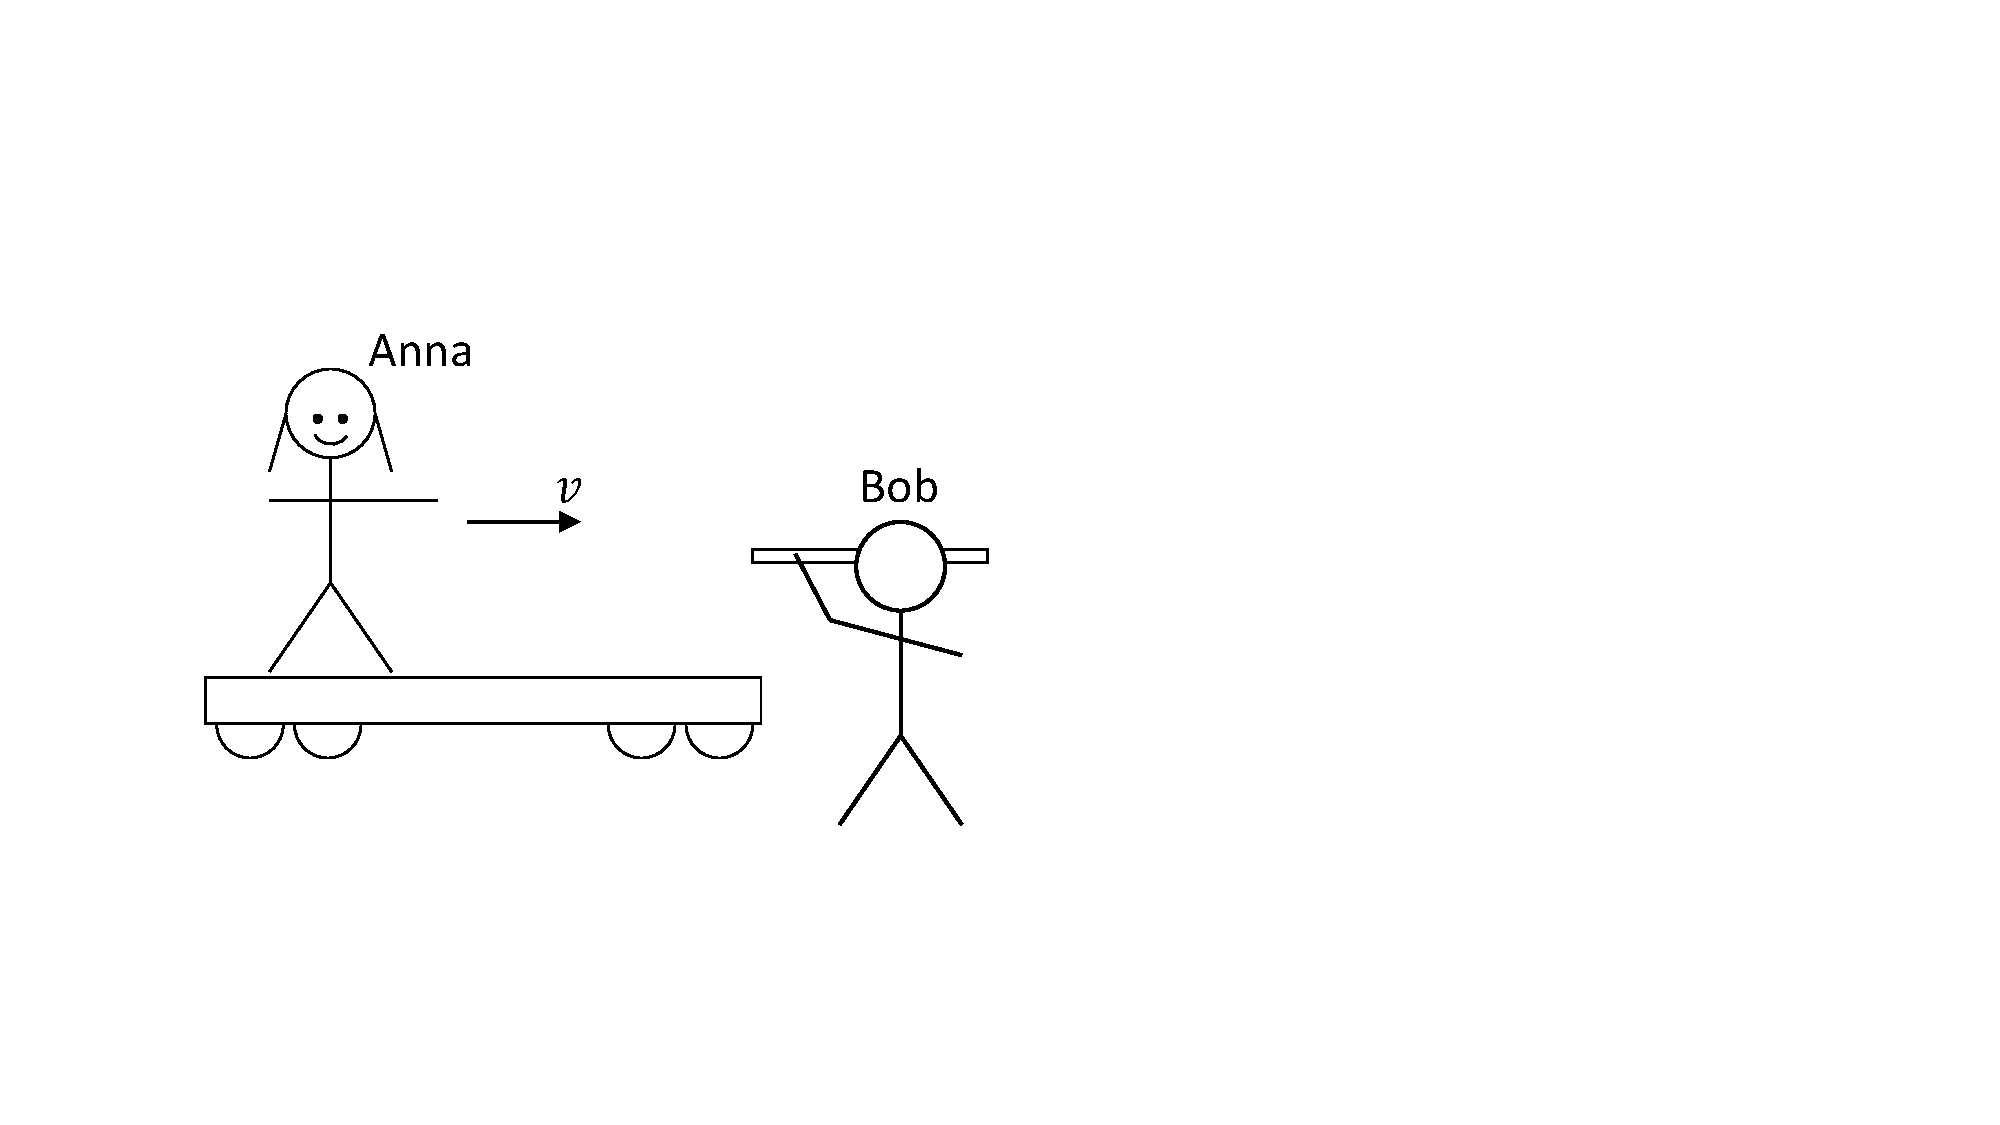
\includegraphics[scale=0.4]{time_dilation_length_contraction/anna_and_bob2.pdf}
\end{center}
\end{wrapfigure}

\textbf{Activity 2: What about Length?}

Anna rides the train again at the same speed, and Bob stands on the side, holding a long rod along the direction of the train tracks.  Bob measures the rod to have length $L_0$.  Bob sees Anna traveling past at speed $v$.  Events ``A'' and ``B'' are Anna's nose being even with the left and right ends of the rod, respectively.  Bob measures the time between event A and event B as $\Delta t=L_0 / v$.  

\begin{enumerate}[labparts, nosep]
\item What does Anna say is their relative speed $v$?  (Same as what Bob measures, bigger, or smaller?)
\answerspace{0.4in}
\end{enumerate}

\begin{enumerate}[labparts, nosep,resume]
\item In Anna's frame, what is the time between events A and B, in terms of $\gamma$ and Bob's $\Delta t$?  (Hint: which of the two observers measures the proper time between the two events?  
\answerspace{0.4in}

\item What does Anna infer is the length $L$ of the rod?  (Answer in terms of $L_0$ and $\gamma$.)
\answerspace{0.4in}

\item Bob's measurement, $L_0$, is the ``proper length'' of the rod.  Write a definition of ``proper length'' that highlights why Bob's measurement is different from that made in any other reference frame.
\answerspace{0.5in}
\end{enumerate}

